\chapter{Data Aggregation Background} % (fold)
\label{cha:Data Aggregation Background}

	Data aggregation has been put forward as an essential paradigm for wireless routing in sensor networks \cite{krishnamachari2002impact}. 
	The idea is to combine the data coming from different sources enroute eliminating redundancy, minimizing the number of transmissions and thus saving energy.
	This paradigm shifts the focus from the traditional address-centric approaches for networking (finding short routes between pairs
	of addressable end-nodes) to a more data-centric approach (finding routes from multiple sources to a single destination that allows in-network consolidation of redundant data).

	One of the fundamental and indispensable functionalities of sensor networks is the ability to answer queries over the data acquired by the sensors. 
	For example, in Figure \ref{fig:Routing River} the base station might be at the end of the river who initiates the query to the sensor network.
	And all the sensor nodes on both sides of the river has to response to the queries of the base station.
	The transreceiver module in the sensor nodes have the limited transreceiving range. 
	The sensor nodes can not communicate to the base station in peer-to-peer fashion.
	The sensor nodes have to communicate via hop-by-hop to the base station.
	This resource constraint forces us to design distributed protocol for sensor networks.  
	\begin{figure}[h!]
		\centering
		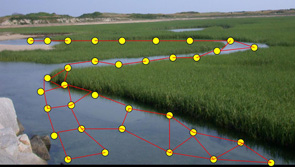
\includegraphics[scale = 2]{images/routing-river.jpg}
		\caption{Routing River \cite{RoutingRiver}}
		\label{fig:Routing River}
	\end{figure}

\section{Data Aggregation}

	The sensor nodes in the network often have limited resources, such as computation power, memory, storage, communication capacity and most significantly, battery power.
	The wireless data communications between nodes consume a large portion of the total energy consumption. 
	In-network data aggregation techniques allow the sensor nodes to aggregate the data before sending it to their parents.
	That reduces the wireless communication happening between the nodes and the overall energy consumption in the network. 	
	For example, in-network data aggregation of the SUM function can be performed as follows.
	All the intermediate sensor nodes in the network, receives the sensor readings from all of its children.
	They aggregate all those readings by applying the summation function to those readings.
	For the star topology shown in Figure \ref{fig:star-network}, the root of the tree receives the following sensor readings $S_{1}(10),S_{2}(14),S_{3}(12),S_{4}(15),S_{5}(11),S_{6}(17)$. And the root has its own reading of $S_{0}(15)$. 
	The root node aggregates all these seven readings and creates an aggregated result as follows:
	\begin{equation}
		S = \sum_{i=0}^6 S_{i}
	\end{equation}
	Now, instead of sending all those sensor readings one at a time to their parent they can send one aggregated sensor reading.
	In this example the aggregate function is summation, but it can be replaced with most of the aggregate function such as (average, median, count) with little or no modification.
	\begin{figure}[h!]
		\centering
		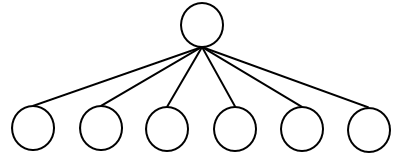
\includegraphics[scale = 1]{images/star-tree.png}
		\caption{Star Network}
		\label{fig:star-network}
	\end{figure}

	According to \cite{zareafifi2012secure}, data aggregation can be defined as follows.
	Consider a sensor network with $n$ sensors collecting data, the data will be propagated in some fashion to the Base Station.
	At the Base Station, the data is aggregated and processed into information. 
	This can be represented as
		$f(x_{1}, x_{2},...,x_{n})$
	where $x_{1}, x_{2},..., x_{m}$ represent the sensor readings.
	Here $f$ is some mapping $f: \mathcal{D}_{1} \times \mathcal{D}_{2} \times ... \mathcal{D}_{n}$ $\rightarrow$ $I$, where $\mathcal{D}_{i}$ represents sensor $i$'s domain and $I$ represents the set of all possible information. 
	Thus the goal is to compute the information as follows:
	\begin{equation}
		\label{eq:aggregation}
		y =\ f(x_{1}, x_{2},...,x_{n})
	\end{equation}

	It is shown that the energy savings achieved by in-network data aggregation are significant \cite{madden2002tag}.
	The in-network data aggregation approach requires the sensor nodes to do more computations.
	But studies have shown that wireless communication of data transmission requires more energy than local computation of the data. 
	In a nutshell, in-network data aggregation is an efficient and a widely used approach for saving bandwidth by doing less wireless communications between sensor nodes and ultimately giving longer battery life to sensor nodes in the network.

	We define the following terms to help us define the goals of in-network data aggregation approach.
	\begin{definition}\label{def:payload}\cite{PayloadWiKi}
		\textbf{Payload} is the part of the transmitted data which is the fundamental purpose of the transmission, to the exclusion of information sent with it such as meta data solely to facilitate the delivery.
	\end{definition}
	\begin{definition}\label{def:information-rate}
		For a given node \textbf {Information rate} is the ratio of the number of sent payloads over the received payloads.
	\end{definition}
	The goal of the aggregation process is to achieve the lowest possible information-rate.
	In the following sections, we show that lowering information-rate makes the intermediate sensor nodes (aggregator) more powerful.
	Also, it makes aggregated payload more fragile and vulnerable to various security attacks.

\section{Bandwidth Analysis}
	Congestion is a widely used parameter while doing bandwidth analysis of networking applications.
	% Picture
	% Definitions vs Equations errors 
	The congestion for any given node is defined as follows:
	\begin{equation}\label{def:congestion}
		Node\ congestion = Edge\ congestion \cdot Fanout
	\end{equation}
	Congestion is a useful factor while analyzing sensor network as it measures how quickly the sensor nodes will exhaust their batteries \cite{madden2003design}. 
	Some nodes in the sensor network have more congestion than the others, the highly congested nodes are the most important to the the network connectivity.
	For example, the nodes closer to the base station are essential for the network connectivity.
	The failure of the highly congested nodes may cause the sensor network to fail even though most of the nodes in the network are alive.
	Hence, it is desirable to have a lower congestion on the highly congested nodes even though it costs more congestion within the overall sensor network.
	To distribute the congestion uniformly across the network, we can construct an aggregation protocol where each node transmits a single payload Defined in \ref{def:payload} to its parent in the aggregation tree.
	In this approach, the fanout ($\delta$) depends on the given aggregation tree.
	For example, an aggregation tree shown in Figure \ref{fig:star-network}, with $n$\ nodes, organized in the star tree topology congestion is $O(n)$.
	And the network organized in the palm tree topology as shown in Figure \ref{fig:palm-tree-network} the congestion is $O(1)$.
	\begin{figure}[h!]
		\centering
		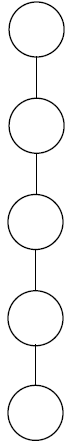
\includegraphics[scale = 1]{images/palm-tree.png}
		\caption{Palm Tree Network}
		\label{fig:palm-tree-network}
	\end{figure}
	This approach can create some highly congested nodes in the aggregation tree which is undesirable.
	In most of the real world applications, we cannot control $\delta$ as the aggregation tree is random.
	Hence, it is desirable to have uniform distribution of congestion across the aggregation tree.

\section{Security Issues}
	Designing secure data aggregation protocol for the wireless sensor network poses a numerous challenges due to resource limitations and inherent characteristics discussed in the previous chapter. 
	As we know, one widely used approach to overcome the bandwidth limitation is to use in-network data aggregation techniques.
	In-network data aggregation approach saves bandwidth by transmitting less payloads between sensor nodes thus increasing the lifetime of the network.
	But that empowers an intermediate aggregate sensor nodes in the network by allowing it to control certain portion of the network.
	The integrity of the aggregated value becomes more valuable.
	A malicious intermediate sensor node who does aggregation over all of its descendants payloads, needs to tamper with only one aggregated payload instead of tampering with all the payloads received from its descendants. 
	Thus, a malicious intermediate sensor node needs to do less work to skew the final aggregated payload.
	An adversary controlling few sensor nodes in the network can cause the network to return unpredictable payloads, making an entire sensor network unreliable.
	Also, an intermediate sensor node becomes more powerful with the increase in number of descendants.

	The aggregation techniques can be compared with compression techniques.
	``Lossy data compression'' is the class of data encoding methods that uses inexact approximations (or partial data discarding) for representing the content that has been encoded. 
	``Lossless data compression'' is a class of data compression algorithms that allows the original data to be perfectly reconstructed from the compressed data.
	The aggregation technique we use is lossy data compression because once the base station receives the final aggregated value it can not create the original sensor readings of the sensor nodes.
	Hence, it is very important the base station has very high confidence in the received final aggregated value. 
	For example, in Equation \ref{eq:aggregation} sensor $2$'s reading is changed from $x_{2}$ (the ``true reading'') to $x'_{2}$ by an intermediate aggregator, then an aggregate node computes $y' =\ f(x_{1},x'_{2},...,x_{n})$.
	It is very likely that $y' \neq y$ where $y$ is the true information if the true reading was counted.
	The base station takes an action based on the received information $y'$.
	How dangerous would it be to act using $y'$?
	Thus, if one ``knows there is some likelihood of false data'' how do we protect the information generated?
	
	Suppose $n$ seismic sensors are collecting seismic readings \cite{zareafifi2012secure}.
	The sensor data is then processed to compute $y = f(x_{1},..., x_{n})$ where $y = (y_{1}, y_{2})$, here $y_{1}$ represents the time prediction of an earthquake and $y_{2}$ represents the duration of the earthquake. Suppose $y^* = (y^*_{1}, y^*_{2})$, where $y^*$ is the approximate (or faulty) information.
	Then to measure the quality we need to compute $|y - y^*|$, but observe that many of the common metrics fail to capture the essence of the prediction (it is more important to determine date than duration).
	Thus a metric that measure the quality of the approximation must make sense. 
	It is possible that the best measure of the essence of the computation does not possess all the	properties of a metric.

	Despite the fact that in-network aggregation makes an intermediate sensor nodes more powerful and aggregated value more vulnerable to various security attacks, some aggregation approaches requires strong network topology assumptions or honest behaviors from the sensor nodes.
	For example, in-network aggregation schemes in \cite{yao2002cougar, madden2003design} assumes that all the sensor nodes in the network are honest. 
	Secure Information Aggregation (SIA) of \cite{przydatek2003sia} enables secure information aggregation such that the user accepts the data with high probability if the aggregated result is within a desired bound, but that the user detects cheating with high probability and rejects the result if it is outside of the bound.
	But SIA provides probabilistic security for the network topology with a single-aggregate model.
	
	Secure hierarchical in-network aggregation (SHIA) in sensor networks \cite{chan2006secure} presents the first and provably secure sensor network data aggregation protocol for general networks and multiple adversaries. 
	We discuss the details of the protocol in the next chapter. 
	SHIA limits the adversary's ability to tamper with the aggregation result with the tightest bound possible.
	But it does not help detecting an adversary in the network.
